\documentclass[11pt,a4paper]{article}
\usepackage[utf8]{inputenc}
\usepackage[T1]{fontenc}
\usepackage[romanian]{babel}
\usepackage[margin=1cm]{geometry}
\usepackage{array}
\usepackage{tabularx}
\usepackage{enumitem}
\setlist{itemsep=2pt,topsep=2pt,parsep=0pt}
\usepackage{graphicx}
\usepackage{setspace}
\usepackage{xcolor}
\usepackage{hyperref}
\usepackage{amssymb}
\setlength{\parindent}{0pt}
\newcommand{\fillline}[1][6cm]{\underline{\hspace{#1}}}
\newcommand{\fillbox}[1][0.4cm]{\framebox[#1]{\rule{0pt}{#1}}}
\newcommand{\checkboxempty}{$\square$}

\begin{document}

\hrule
\vspace{0.15cm}
\noindent
\begin{minipage}[t]{0.40\textwidth}
\vspace{0pt}
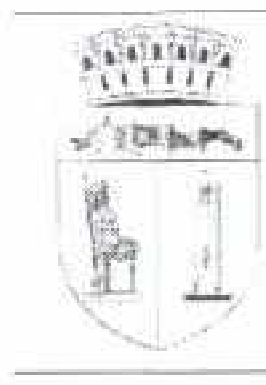
\includegraphics[height=1.5cm]{assets/stema-cluj.png}%
\hspace{0.2cm}%
\raisebox{0.5cm}{\parbox[t]{3.5cm}{\textbf{PRIMĂRIA}\\\textbf{CLUJ-NAPOCA}}}
\end{minipage}%
\begin{minipage}[t]{0.30\textwidth}
\centering
\vspace{0.25cm}

\includegraphics[width=5cm]{assets/barcode-802013.png}
\end{minipage}%
\begin{minipage}[t]{0.30\textwidth}
\raggedleft
\vspace{0.6cm}
Nr. \fillline[3cm] / \fillline[1cm]
\end{minipage}

\vspace{0.2cm}
\hrule
\vspace{0.3cm}

Către,

\begin{center}
\textbf{\underline{DIRECŢIA DE ASISTENŢĂ SOCIALĂ ŞI MEDICALĂ}}\\
\underline{Serviciul Asistenţa Persoanelor cu Dizabilităţi}
\end{center}

\vspace{0.3cm}

\hspace{1cm}Subsemnatul(a) \underline{ {{nume_titular}} } -- CNP \underline{ {{cnp_titular}} } domiciliat(ă) în Cluj-Napoca, str. \underline{ {{strada}} }, nr. \underline{ {{numar}} } ap. \underline{ {{apartament}} }, sunt persoană cu handicap grav / reprezentant legal al persoanei cu handicap grav \fillline[6cm] domiciliat(ă) în Cluj-Napoca, str. \fillline[8cm], nr. \fillline[1.5cm], ap. \fillline[1.5cm].

\vspace{0.2cm}

\hspace{1cm}Grad de handicap: \underline{ {{grad_handicap}} }.

\vspace{0.25cm}

\hspace{1cm}Solicit acordarea \textbf{\textit{indemnizaţiei lunare}}, conform art. 42, alin. (4) din Legea nr. 448 / 2006 privind protecţia şi promovarea drepturilor persoanelor cu handicap, republicată, cu modificările și completările ulterioare.

\vspace{0.25cm}

\hspace{1cm}De asemenea, mă oblig să aduc la cunoştinţă, \textbf{în termen de 48 de ore}, orice modificare survenită în situaţia persoanei cu handicap, cu privire la gradul de handicap, domiciliu, reşedinţă şi alte situaţii de natură să modifice acordarea indemnizaţiei mai sus menţionate.

\vspace{0.25cm}

\hspace{1cm}În cazul în care nu respect obligaţiile voi suporta rigorile legii.

\vspace{0.25cm}

Tel. de contact \underline{ {{telefon}} }

\vspace{0.3cm}

\begin{itemize}[leftmargin=*,label=\checkboxempty]
\item Prin prezenta solicit comunicarea răspunsului pe următoarea adresă de e-mail:\\
\underline{ {{email}} }
\item Mă oblig să comunic instituției orice modificare intervine în legătură cu această adresă de e-mail
\item Îmi exprim consimțământul ca Primăria Municipiului Cluj-Napoca să comunice orice informații, date personale, clarificări și completări pe adresa de e-mail indicată mai sus
\item Am luat la cunoștință faptul că în cazul nefuncționării serverului de e-mail comunicat sau în cazul adresei greșite de e-mail, Municipiul Cluj-Napoca nu poate fi tras la răspundere pentru acest lucru
\end{itemize}

\vspace{0.3cm}

Solicit plata indemnizației lunare prin: \underline{ {{modalitate_plata}} }

\vspace{0.3cm}

\begin{itemize}[leftmargin=*,label=\checkboxempty]
\item virament bancar
\item mandat poștal
\item casierie
\end{itemize}

\vspace{0.3cm}

IBAN (dacă virament bancar): \underline{ {{iban}} }

\vspace{1.5cm}

Data: \fillline[3cm] \hfill Semnătura: \fillline[4cm]

\vspace{0.25cm}

\hrule
\vspace{0.2cm}
\small
http://dasmclujnapoca.ro\\
telefon/e-mail: 0264599316 / dizabilitati@dasmclujnapoca.ro\\
Cluj-Napoca, str. Venus FN între 20-22

\vspace{0.3cm}
\hrule
\vspace{0.2cm}
www.primariaclujnapoca.ro\\
telefon: 0264/596.030\\
Cluj-Napoca, str. Moţilor, nr. 3 \hfill \textbf{
\includegraphics[width=4cm]{assets/barcode-802013.png}}

\vspace{0.2cm}
\hrule
\vspace{0.2cm}
\scriptsize
Timp estimativ de completare: \textbf{5 minute}\\
Datele personale care vă sunt solicitate prin prezenta cerere vor fi prelucrate numai în vederea procesării și soluționării solicitării dumneavoastră. Primăria municipiului Cluj-Napoca garantează securitatea procesării datelor și arhivarea acestora în conformitate cu prevederile legale în vigoare. Responsabilul Primăriei municipiului Cluj-Napoca cu protecția datelor poate fi contactat pe adresa de email dpo@primariaclujnapoca.ro.\\
În conformitate cu Regulamentul nr. 679/2016 aveți dreptul de a solicita Primăriei municipiului Cluj-Napoca, în ceea ce priveşte datele cu caracter personal referitoare la persoana vizată, accesul la acestea, rectificarea sau ştergerea acestora sau restricţionarea prelucrării sau a dreptului de a vă opune prelucrării, precum şi a dreptului la portabilitatea datelor.

\end{document}
